\documentclass[12pt,twoside]{extarticle}
\usepackage{lmodern}


\usepackage[T1]{fontenc}
\newcommand{\changefont}[3]{\fontfamily{#1}\fontseries{#2}\fontshape{#3}\selectfont}
\changefont{ppl}{m}{n}

\usepackage{color}
\usepackage{amsmath}
\usepackage{graphicx}
\usepackage{amssymb}
\usepackage{esint}
\usepackage[utf8x]{inputenc}
\usepackage{fullpage}


\usepackage[hmarginratio=1:1,top=32mm,left=22mm]{geometry} % Document margins


\usepackage{xcolor} % Required for specifying colors by name
\definecolor{daliblue}{RGB}{51,51,153} % Define daliblue-color used for highlighting throughout the document
\definecolor{dalifile}{RGB}{217,231,247} %

%define boxes with background colors
\usepackage[framemethod=default]{mdframed}
% Exercise box	  
\newmdenv[skipabove=7pt,
skipbelow=7pt,
rightline=true,
leftline=true,
topline=false,
bottomline=false,
backgroundcolor=daliblue!10,
linecolor=daliblue,
innerleftmargin=5pt,
innerrightmargin=5pt,
innertopmargin=5pt,
innerbottommargin=5pt,
leftmargin=0cm,
rightmargin=0cm,
linewidth=4pt]{eBox}	


\newmdenv[skipabove=7pt,
skipbelow=7pt,
rightline=true,
leftline=true,
topline=true,
bottomline=true,
backgroundcolor=dalifile!30,
linecolor=dalifile,
innerleftmargin=5pt,
innerrightmargin=5pt,
innertopmargin=5pt,
innerbottommargin=5pt,
leftmargin=0cm,
rightmargin=0cm,
linewidth=4pt]{fBox}	



\newenvironment{exercise}{\begin{eBox}}{\hfill{\color{daliblue}}\end{eBox}}
\newenvironment{file}{\begin{fBox}}{\hfill{\color{dalifile}}\end{fBox}}



\setlength{\parindent}{0cm}
\setlength{\headheight}{10pt}% offset of header from top margin
\setlength{\headsep}{0.5cm}% offset of main text from header


\usepackage{fancyhdr} % Headers and footers

\pagestyle{fancy} % All pages have headers and footers
\fancyhead{} % Blank out the default header
\fancyfoot{} % Blank out the default footer
\fancyhead[C]{DALI manual $\bullet$ Ln(a) Sellentin } % Custom header text
\fancyfoot[RO,LE]{\thepage} % Custom footer text


\begin{document}
\thispagestyle{empty} % All pages have headers and footers
 
\begin{center}
\begin{LARGE}
\vspace{6cm}
 \textsc{DALI MANUAL\\\vspace{0.5cm}Bending and Flexing Fisher Matrices}
 \vspace{1cm}
\end{LARGE}

Ln(a) Sellentin\\Institut für Theoretische Physik\\Universität Heidelberg\\
sellentin@stud.uni-heidelberg.de\\
\vspace{0.5cm}
 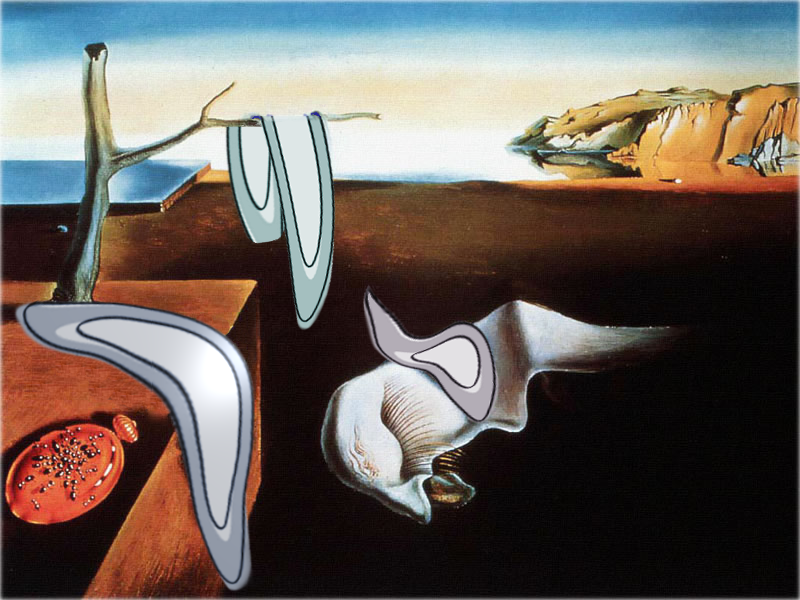
\includegraphics[width=\textwidth]{Dali.png}
\end{center}

\newpage
\thispagestyle{fancy}
 


\vspace{3cm}

\section{Manual of the Manual}
\begin{itemize}
 \item Please read the manual and use the DoxyDocumentation. If you don't get along with the code, please complain to the author about the manual and the documentation. Obviously there is never an end to maintaining and improving a code and a manual, so feedback is very welcome and the documentation will improve significantly if other users comment.

For visual purposes we use the following two items:

 \begin{exercise}
 This is a terminal
 \end{exercise}

\begin{file}
This is some file.
\end{file}
\end{itemize}


\section{Doxygen}
The code also has a doxygen documentation. Please open any of the html files in the directory DoxyDocu.\\
All members and member functions are visible in doxygen. However, only functions that the user typically needs also have a doxygen description. They appear in blue and you can click on them. If you want to see how DALI works under the hood, you'll find more comments in the code itself, and you can use the doxygen search-engine in order to find your way around.

\section{Dependencies}
The code has been tested with Ubuntu 13.10 and 14.05 and Debian 7.8 and runs flawlessly and without memory leaks under the following conditions:
\begin{itemize}
\item the compiler g++ should be version 4.7.2
\item python is installed, together with the matplotlib, numpy and scipy (Python is needed for plotting only.)
\item the Gnu Scientific Library (GSL, 1.16+dfsg-1 or similar versions) is installed in the standard search path of your compiler. Else, you will have to modify the example makefile and tell g++ where to find the GSL.
\item Once you have everything installed, you can test DALI:
\begin{exercise}
 cd ./Examples \\
 make gen  \textcolor{daliblue!70}{\hspace{0.7cm}(Should compile nicely if everything is okay.)}\\
 ./gen \\
\end{exercise}

\end{itemize}


\section{In which cases can DALI be used?}
\begin{itemize}
 \item You need to know the maximum likelihood point: either because you do a forecast, such that you can decide where your exemplary likelihood will peak, or you work with any kind of mock data, or you work on real data but already know where the peak is. DALI is using the maximum likelihood point as expansion point for the approximation.
\item The measurement errors are Gaussian, or can be made Gaussian via the Central Limit Theorem by binning.
\end{itemize}



\section{Tutorials}
Currently, two programms are included, that will explain you further how to approach DALI:
\begin{itemize}
 \item Open a terminal, cd to the directoy in which the makefile lies
\item type
\begin{exercise}
 make tutorial
\end{exercise}

\item Watch whether DALI compiles nicely. If no warnings occur, it did.
\item After successfull compilation type 
\begin{exercise}
 ./tutorial
\end{exercise}
\item the tutorial will explain you how to use DALI
\item An example of how I used DALI is given by 'TestGen.cpp'
\item Look at that file for inspiration, if you want to execute it:
\begin{exercise}
 make gen\\
 ./gen
\end{exercise}
\item This will draw approximations to the boxy ring from (arXiv xyz)
\item Documentation of single functions can be found in the doxygen-docu
\item how to load Dali tensors from a file can be seen in LoadGenFromFile.cpp
\end{itemize}



\section{Terminology}
The code approximates a Gaussian likelihood
\begin{equation}
 L = \frac{1}{\sqrt{(2\pi)^n |C|}} \exp\left(-\frac{1}{2} (\vec{d} -\vec{m}) C^{-1}  (\vec{d} -\vec{m}) \right)
\end{equation}
where
\begin{equation}
\vec{m}= \vec{m}(p_1, p_2,...., x_1,x_2...)
\end{equation}
is the prediction of the data set $\vec{d}$. The prediction is the mean of the data and can depend on the parameters $p_1,p_2...$, which shall be measured, and some other independent variables $x_1,x_2....$. The code calls $\vec{m}$ \emph{PhysMod}, as an abbreviation of 'physical model, that quantifies the measurement'. The covariance matrix $C$ includes all the errors (systematic and measurement errors). The code calls $C$ \emph{DataCovMatrix}.

Some other terms that appear throughout the code:
\begin{itemize}
 \item Dali-tensors: these are the higher dimensional equivalents of the Fisher matrix. In our papers, they are denoted by $S_{\alpha\beta\gamma}, Q_{\alpha\beta\gamma\delta}$... the code computes these automatically.
 \item the model: this is your numerical prediction of how the data will look like.
\item independent variables: all variables that the data depend on, but that are not theoretical parameters. The distinction between independent variables and theoretical parameters seems to be tricky to understand, so here is what sets the two apart:
\begin{itemize}
\item The code cannot derive with respect to independent variables.
\item The code will derive with respect to all theoretical parameters.
\item The data might depend on some input values with respect to which the user does \emph{not} want to derive. Hence, the independent variables were created.
\item Everything that shall appear on the axes of a confidence contour plot will be a theoretical parameter.
\end{itemize}
Example: You breed zebrafish (danio rerio) for brain scans or other scientific purposes. These fish multiply at a rate $\Gamma$ which depends on theoretical parameters like the amount of magnesium ($n_{mg}$) and potassium $(n_K)$ in the fish food. The fish will furthermore sadly die at a constant rate $\Gamma^\dagger$, due to their finite lifetime. In case you never run out of fish food and storage room for the water tanks, you'll have $$N(t) = N_0 \exp\left((\Gamma(n_{mg},n_K) -\Gamma^\dagger) t\right)$$ fishes at any point in time. Let's assume you bought some fish food, which does not tell you how much potassium and magnesium it contains. So you try to estimate it by measuring the curve $N(t)$. In this setup $n_{mg}$ and $n_K$ are \emph{parameters} (since you want to measure them), and the time \emph{t} is your independent variable. We 
call it independent, since it is up to you, how to choose the different measurement points in $t$. You might measure today and tomorrow, but you might also choose to count your fish today, in two weeks and in three weaks.
For DALI, everything that you can control, and which you don't need to measure, is an independent variable: these are all quantities that your model depends on, but that shall not be measured. In case of the fishes, you might happen to know that your measurement of $n_{mg}, n_K$ gets better if you also include a second independent variable which you can control: For example the water temperature $T$, such that you have $N(t,T, n_{mg}, n_K)$. Then you start to vary the temperature, and measure at different points in time, and at different temperatures. The mere fact that you can control the temperature, makes it an independent variable. Be aware that your likelihood will change shape, if you modify your grid of independent variables. (In the code, you have to specify them in \emph{datavaribs} and the number of data points is called \emph{noofdat}).
\item parameters: these are all the parameters which you want to constrain by comparing to data. The code will derive your functions with respect to these parameters. These are the quantities that are not controllable/known, once real data are analyzed.
\end{itemize}






\section{Tips for users that are new to c/c++}
C/C++ is not to everyone's taste, and you do not need to be a c++ freak in order to use DALI. For your convenience, here are the basic functionalities, which you might or might not want to look up.

\begin{itemize}
\item vectors: c++ vectors can dynamically change in size. DALI uses them to allocate space for the data set, the parameters and similar quantities, of which every user will have a different number. The main functionalities which you need to be familar with are the allocation of a c++ vector and how to assign values to it's elements. Examples can be found in the example codes. For further reference please ask Google. You'll need to understand the operator $[]$ and the operator $=$ and potentially \emph{resize()} which tells a vector how many elements it can take. c++ starts counting at zero.\\
Example:\\
\begin{file}
(in some file named examplefile.cpp....)\\
\#include<vector>\\
using namespace std;\\

int main()\\
\{\\
 vector<double> smallvector;\\
 smallvector.resize(2);\\
 smallvector[0] = 2.718;\\
\}\\
\end{file}

\item (pure) virtual functions: it is basically a place holder for a not-yet existing function. DALI expects you to overwrite these virtual functions with functions that specify your physical application. If you do not overwrite it, g++ will give you lengthy error messages that somewhere contain the word \emph{virtual}. This basically tells you that the code does not compile, since it's central asset is missing: this will happen if you did not tell the code what the covariance matrix looks like, and what your physical model is.
\item Dali uses the GNU Scientific Library (GSL), which knows how to deal with matrices, vectors, how to diagonalize them, and so on. The GSL is also used to draw random numbers. The GSL manual details the use of these functions.
\item pointers: pointers enter DALI through the GSL. The syntax
\begin{file}
 $pointer = 0;$
\end{file}
does not set the variable to zero, to which the pointer points! It creates a nullpointer instead. You'll not need to understand the difference, if you don't play around in the source code.
\item If the code does something unexpected, or gets stuck, please put it into the debugger \emph{gdb}. The syntax is\\
\begin{exercise}
 gdb ./yourdaliexecutable\\
break DaliGen.cpp:3                   \textcolor{daliblue!70}{//if you want to break at line 3 of the source code DaliGen.cpp}\\
run                                   \textcolor{daliblue!70}{//starts code}\\
backtrace                             \textcolor{daliblue!70}{//tells you, how the code got to the breakpoint. Please \emph{read} what gdb tells you!}\\
\end{exercise}
You can exit gdb by typing q.
\end{itemize}





\section{Structure of the code}
If you use DALI, you will be interested in calculating DALI tensors, and in plotting resulting likelihoods. Calculating the tensors can take some time, and is rather independent of plotting. Therefore, DALI uses two classes \emph{DaliGen} and \emph{DaliPaint} which deal with the both main tasks. \emph{DaliPaint} allows you to load Dalitensors from files, to store and to load MCMC chains, it plots Fisher-ellipses and non-Gaussian likelihood contours. You'll probbaly use the functionalities of this class without an changes- \emph{DaliGen} is the class that you have to adapt to your own physical application. You do this by \emph{derivation}. This will keep the DALI source code nicely separated from your own code. If you simply use DALI, you'll never have to edit any of the provided DALI source code from the folder \emph{source}. In order to learn how to derive your own application, have a look at the folder \emph{examples}. 

\begin{itemize}
\item The class \emph{DaliGen}: you will derive from this class, in order to specify DALI to your problem. You don't need to understand c++-derivation. Simply use the examples given in the tutorial, and overwrite the functions that tell you that you shall overwrite them. In order to do this, open the file \emph{Tutorial.cpp}, go to the terminal, cd to your dali-folder and type\\
\begin{exercise}
 make tutorial\\
./tutorial\\
\end{exercise}
This will print messages to the screen of what DALI wants you to do. Edit your Tutorial.cpp accordingly. (You might want to keep a backup.)
\item The class \emph{DaliPaint}: You'll use this class to MCMC sample the likelihood-approximation or to plot it on a grid. This class can also load Dali tensors from files. It works independent of the DaliGen class, but you can pass tensors of a DaliGen-object to a DaliPaint object in the main(). It also allows you to add Dali-Tensors of different experiments, just like onw would do when adding Fisher matrices of different experiments.
\item \emph{Utils.cpp} and \emph{Utils.h}: contains some random mathematical utilities that DALI uses, but that other codes could also be interested in. E.g. taking the trace of a matrix, calculating where confidence contours lie and so on. You might find it interesting, but you'll probably not need it.
\item The class \emph{DaliBase} contains functionalities that all Dali-Object will find handy: it can derive your physical model with respect to parameters and print out informations. You'll probably not care about its files \emph{DaliBase.h} and \emph{DaliBase.cpp}. These are only needed by DALI internally.
\end{itemize}


\section{Dos and Don'ts}
\begin{itemize}
\item Do: Derive your own class from the DaliGen or DaliConst classes.
This is done outside the main() function.
\item Don't: If you are in the main() function, never type something
like\\
\begin{file}
 DaliGen.DeclareData();\\
\end{file}
You should never have any 'DaliGen' or 'DaliBase' or 'DaliPaint' written in your main(). The compiler will be angry and complain that you did not overwrite pure virtual functions. The reason is that you confused the classes DaliGen, and DaliPaint with an \emph{object} of them.
\item Do instead: Create a derived object of them. So in the main it will look like\\
\begin{file}
 MyOwnDaliSpecialzedObject.DeclareData();\\
\end{file}
Where MyOwnDaliSpecializedObject is the class that you yourself have created:
it contains all of your problem-specific functions (data set, physical
model, covariance matrix). See tutorials for more details on the syntax.
\item Don't forget that your covariance matrix has the dimensions of
your data set! Not the dimensions of your parameter space. It is
therefore explicitely called DataCovMatrix, in order to remind users.
\item Plot your derivatives. These are the essential assets from which DALI computes the likelihood contours. If the derivatives are wrong, the likelihood contours will also be wrong. The code contains the functions \emph{PrintFirstDmod()} for writing the first derivatives to a file, and similar functions for the higher order derivatives. It can also write the derivatives of the diagonal of the covariance matrix to a file if you call \emph{ConductRecommendedChecks(2)} at the beginning of your code. The code will not write out all derivatives of the non-diagonal elements of the covariance matrix: if you do this for a covariance matrix of 5000 data points... and ten parameters... you will end up with huge files. Users who do need to plot the derivatives of huge covariance matrices are advised to come up with a low-memory solution for such cases... 
If you want to plot a small non-diagonal covariance matrix and its derivatives, the code is able to do that: you just need to decomment the respective lines in the function \emph{PlotMatrix}.
\end{itemize}

\section{Tips}
\begin{itemize}
\item a c++ class has member functions and member variables. If you are a C-programmer, you might wonder where to put your global structs. Especially, if you use the GSL, which enforces recasts of void-pointers, you might wonder where to put the param-structs of the GSL. Here is how it worked in all cases that were tried so far: global structs of a running C-code remain global structs. If you create pointers of a struct, malloc them in the main() as usual. Your derived DaliGen object is then given one of these pointers. You might want to give your DaliGen-class a member variable that is a pointer to your specific global struct.
 \item If your plots look bad, don't increase brutally the number of MCMC samples. Often you will have much better results by changing the binwidths and the proposal distribution for the sampler. If they then still look bad, increasing the samples will be the last option.
 \item Sometimes the c++ code executes fine - but in between, python prints huge error messages to the screen, and then c++ continues happily. Of course, this can only happen if you call python from your c++main():
 \begin{file}
  system("python executethis.py");
 \end{file}
If that happens, open the python files and see what is the matter.
\end{itemize}


\section{FAQ}

\subsection{DALI runs nicely but suddenly my computer stops responding. Why?}
This sounds like a memory leak. DALI itself does not leak memory but if you overwrite one of its virtual functions with a leaky function, then very quickly, your computer can run out of memory: Imagine the function that you provided for \emph{DataCovMat} leaks memory, and you have a dataset of 1000 points. DALI will then call the function \emph{DataCovMat} at least $5\cdot 10^5$ times to fill all the entries of the covariance matrix, and even more often if it also takes derivatives of the matrix. If your function leaks memory each time, then you start to exhaust your RAM, your computer will start swapping and you notice that it stops responding. So make sure all functions that you provide, do not leak memory. You can check this for example with \emph{valgrind}.

\subsection{My plot looks something like this, what is happening?}
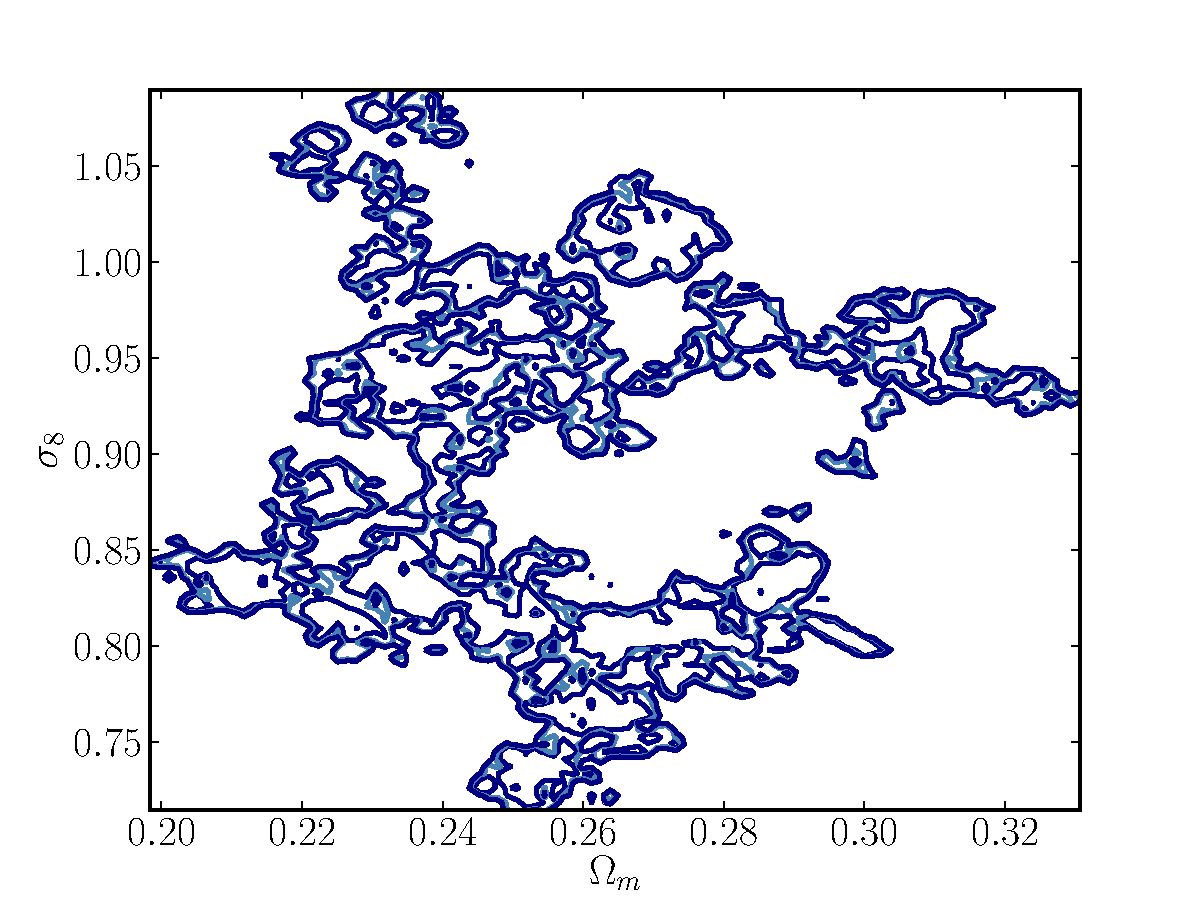
\includegraphics[width = 0.6\textwidth]{0101.pdf}\\
Basically, this happens if the MCMC sampler doesn't work properly. There are various possible reasons for this behaviour:
\begin{itemize}
 \item Did you pass the Dali tensors correctly to the DaliPaint object? 
\item Are the derivatives calculated correctly? If you use a too small step for the finite differences, the derivatives will be noisy. This then corrupts your DALI-tensors and thereby the likelihood. Try to increase the step size in this case. Write out the derivatives with the functions provided by \emph{DaliBase} and plot them to see what is going on.
\item You might have not enough samples in a highdimensional paramater space, and the marginalization produces these weird islands.
\end{itemize}




\section{Related publications}
The framework behind DALI was presented in the publications
\begin{itemize}
 \item \textsc{Forecasting with higher order Fisher matrices}, E. Sellentin, M. Quartin, L. Amendola, arXiv: 1401.6892, MNRAS (2014), 441
\item Title to be determined in arxiv 'when synchronized with the group'
\item DALI-weak lensing for Euclid in arxiV 'when Bjoern and I find time simultaneously'
\end{itemize}





 
 
 
 
\end{document}
